We next classify a single transformation, first by its fixed points and then by the motion it produces. Its fixed points and displacement will later distinguish the geometric terms in a trace formula. The boundary used here is $\partial\mathbb H=\mathbb R\cup\{\infty\}$, with the usual fractional action extended to poles and infinity.

\begin{definition}[The three nonidentity types]\label{hyperbolic.types}
Let $g\in G\setminus Z$. Its effective transformation is called elliptic, parabolic, or hyperbolic according as
\[
 D(g)=(\operatorname{tr}g)^2-4
\]
is negative, zero, or positive. This definition is independent of the lift $g$ or $-g$. Elements of $Z$ give the identity transformation and are excluded from the parabolic case.
\end{definition}

\begin{proposition}[Classification by fixed points]\label{hyperbolic.fixed-point-classification}
Let $g\in G\setminus Z$. Its effective transformation is:
\begin{itemize}
\item elliptic if and only if it has exactly one fixed point in $\mathbb H$; in this case it has no fixed point on $\partial\mathbb H$;
\item parabolic if and only if it has exactly one fixed point on $\partial\mathbb H$; in this case it has no fixed point in $\mathbb H$;
\item hyperbolic if and only if it has exactly two fixed points on $\partial\mathbb H$; in this case it has no fixed point in $\mathbb H$.
\end{itemize}
\end{proposition}

\begin{proof}
Write $g=\begin{smallpmatrix}a&b\\c&d\end{smallpmatrix}$. A finite fixed point satisfies $(az+b)/(cz+d)=z$, hence
\begin{equation}\label{eq:mobius-fixed-point}
 cz^2+(d-a)z-b=0.
\end{equation}
No root of this equation is a pole: if $cz+d=0$ and the equation held, then also $az+b=0$, contradicting $ad-bc=1$. Infinity is fixed exactly when $c=0$.

Suppose first that $c\ne0$. The fixed-point equation \eqref{eq:mobius-fixed-point} is quadratic, with discriminant
\[
 (d-a)^2+4bc=(a+d)^2-4(ad-bc)=(\operatorname{tr}g)^2-4=D(g).
\]
If $D(g)<0$, its roots are a nonreal conjugate pair, so exactly one lies in $\mathbb H$ and neither lies on the boundary. If $D(g)=0$, there is exactly one root, which is real. If $D(g)>0$, there are exactly two roots, both real. Infinity is not fixed in any of these cases.

It remains to treat $c=0$, when infinity is fixed. Now $ad=1$ and $D(g)=(a-d)^2\geq0$. If $D(g)=0$, then $a=d=1$ or $a=d=-1$. Since $g\notin Z$, we have $b\ne0$, and the fixed-point equation reduces to $-b=0$, which has no solution. Infinity is therefore the only fixed point. If $D(g)>0$, then $a\ne d$, and the equation has the single finite root $b/(d-a)\in\mathbb R$, in addition to infinity. These cases exhaust the possible signs of $D(g)$ and give both directions of each assertion.
\end{proof}

\phantomsection\label{hyperbolic.normal-forms}
We now choose coordinates adapted to the fixed points. Conjugating by $h\in G$ replaces $g$ by $hgh^{-1}$ and carries each fixed point $p$ to $h\cdot p$. The following three results describe the resulting motions.

\begin{proposition}[Elliptic transformations are rotations]\label{hyperbolic.elliptic-normal-form}
Every elliptic transformation is conjugate in $\overline G$ to the action of $k(\theta)$ for some $\theta\notin\pi\mathbb Z$. In disk coordinates centered at its fixed point, this action is the rotation $\zeta\mapsto e^{2i\theta}\zeta$.
\end{proposition}

\begin{proof}
Let $p\in\mathbb H$ be the unique fixed point. Choose $h=s(p)^{-1}$, so $h\cdot p=i$. Then
\[
 (hgh^{-1})\cdot i=h\cdot(g\cdot p)=h\cdot p=i.
\]
The \hyperref[hyperbolic.stabilizer]{stabilizer of $i$} is $K$, so $hgh^{-1}=k(\theta)$ for some real $\theta$. Since conjugation cannot turn a noncentral matrix into a central one, $k(\theta)\ne\pm I$, or equivalently $\theta\notin\pi\mathbb Z$.

For an arbitrary point $z\in\mathbb H$, use the disk coordinate $\zeta=C(h\cdot z)$. The Cayley rotation formula \eqref{eq:cayley-rotation} gives
\[
 C(h\cdot(g\cdot z))
 =C(k(\theta)\cdot(h\cdot z))
 =e^{2i\theta}C(h\cdot z)=e^{2i\theta}\zeta.
\]
Thus this coordinate turns the transformation into an ordinary rotation of the disk about $0$.
\end{proof}

The \hyperref[hyperbolic.elliptic-motion-diagram]{elliptic diagram} shows why the choice of model matters. Rotation is Euclidean rotation in the disk; its image in the half-plane follows curves around the interior fixed point. The curves shown are the continuous orbits of the rotation subgroup. A single transformation moves a point by one fixed angle along such a curve.

\begin{figure}[htbp]
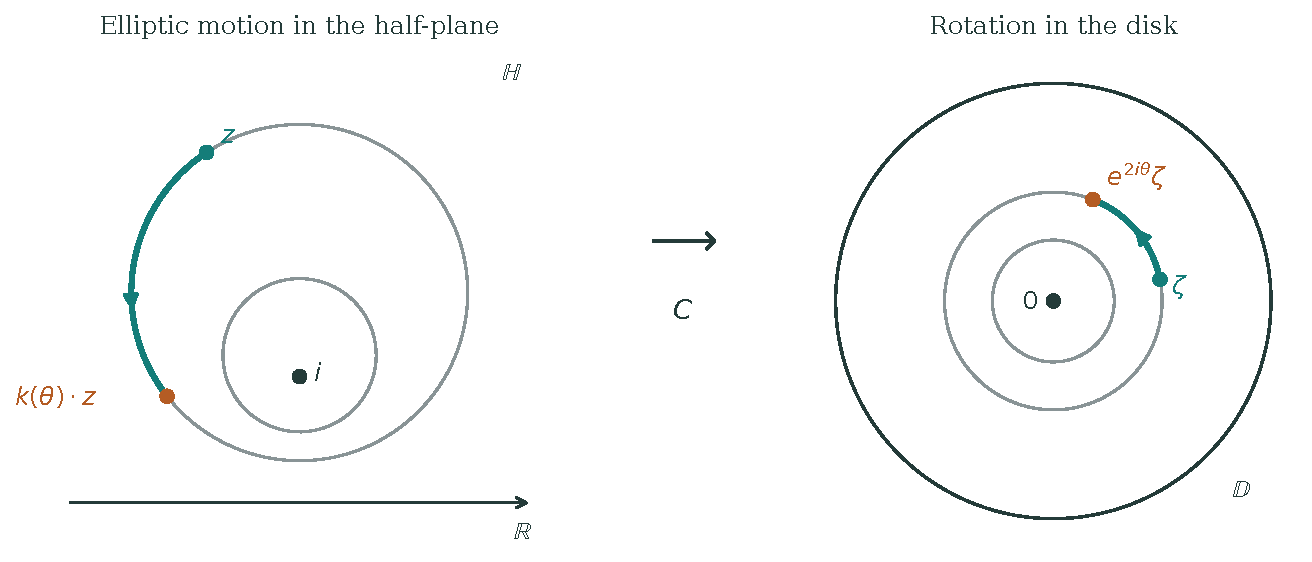
\includegraphics[width=\linewidth]{volumes/Volume01/A/chapters/Chapter01/sections/Section05/figures/elliptic-motion.pdf}
\caption{An elliptic motion with fixed point $i$, shown in the half-plane and after the Cayley map. Corresponding marked points have the same color. In the disk, the motion is rotation through $2\theta$ about $0$. The half-plane curves are the inverse images of circles centered at $0$ in the disk; they are not geodesics.}
\label{hyperbolic.elliptic-motion-diagram}
\end{figure}

\begin{proposition}[Parabolic transformations are translations]\label{hyperbolic.parabolic-normal-form}
Every parabolic transformation is conjugate in $\overline G$ to $z\mapsto z+t$ for some real $t\ne0$. In these coordinates its unique boundary fixed point is infinity.
\end{proposition}

\begin{proof}
Let $p\in\partial\mathbb H$ be its unique fixed point. If $p=\infty$, take $h=I$. Otherwise $p\in\mathbb R$, and the determinant-one matrix
\[
 h=\begin{pmatrix}0&-1\\1&-p\end{pmatrix}
\]
acts by $z\mapsto-1/(z-p)$ and sends $p$ to infinity. Thus $hgh^{-1}$ fixes infinity and has the form $\begin{smallpmatrix}a&b\\0&d\end{smallpmatrix}$, with $ad=1$.

There is no finite fixed point. Its fixed-point equation is $(d-a)z-b=0$, so $d=a$; otherwise it would have a real solution. Hence $a=d=\varepsilon$ for $\varepsilon\in\{1,-1\}$, and $b\ne0$ because the transformation is not the identity. Its action is
\[
 z\longmapsto\frac{\varepsilon z+b}{\varepsilon}=z+t,
 \qquad t=b/\varepsilon\ne0.
\]
Multiplying the lift by $\varepsilon I$ identifies it with $n(t)$ in $\overline G$. The sign of $t$ specifies the direction of translation; we do not impose $t>0$.
\end{proof}

The \hyperref[hyperbolic.parabolic-motion-diagram]{parabolic diagram} shows the horizontal motion in these coordinates.

\begin{figure}[htbp]
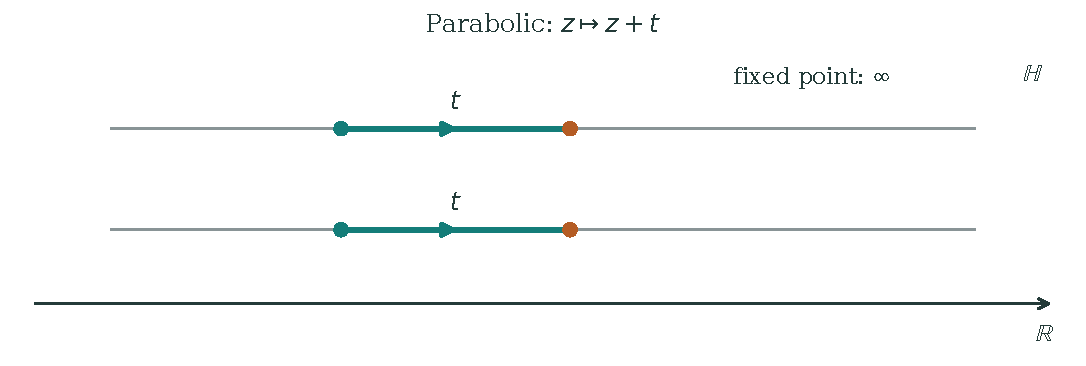
\includegraphics[width=\linewidth]{volumes/Volume01/A/chapters/Chapter01/sections/Section05/figures/parabolic-motion.pdf}
\caption{The parabolic normal form $z\mapsto z+t$, illustrated for $t>0$, moves points horizontally and fixes only infinity on the boundary. The horizontal lines are trajectories of the translation subgroup; they are not geodesics. Infinity lies outside this finite coordinate window.}
\label{hyperbolic.parabolic-motion-diagram}
\end{figure}

\begin{proposition}[Hyperbolic transformations are dilations]\label{hyperbolic.hyperbolic-normal-form}
Every hyperbolic transformation is conjugate in $\overline G$ to $z\mapsto e^r z$ for some $r>0$. In these coordinates its boundary fixed points are $0$ and $\infty$.
\end{proposition}

\begin{proof}
The characteristic polynomial of $g$ is $X^2-(\operatorname{tr}g)X+1$. Since its discriminant $D(g)$ is positive, it has two distinct real roots whose product is $1$. They have the same sign. Replacing $g$ by $-g$ if necessary gives a lift with positive eigenvalues $\lambda,\lambda^{-1}$, where $\lambda>1$.

Choose real eigenvectors for $\lambda$ and $\lambda^{-1}$ in that order, and use them as the columns of a matrix $P$. They are independent. Change the sign of one column if necessary so that $\det P>0$, then divide both columns by $\sqrt{\det P}$. The resulting matrix still has those eigenvectors as columns and now lies in $G$. Thus
\[
 P^{-1}gP=\begin{pmatrix}\lambda&0\\0&\lambda^{-1}\end{pmatrix}
\]
for the chosen lift. Its fractional action is $z\mapsto\lambda^2z$. Put $r=2\log\lambda>0$, so $\lambda^2=e^r$. This action fixes $0$ and infinity. The choice of eigenvector order places the attracting fixed point at infinity.
\end{proof}

The geometry of this normal form is shown in the \hyperref[hyperbolic.translation-dilation-diagram]{hyperbolic axis diagram}. Put $h=P^{-1}$ for the conjugating transformation in the proof. The dilation preserves the positive imaginary axis, and $h^{-1}$ carries it to the geodesic joining the two fixed points of $g$. When both fixed points are finite, this geodesic is the semicircle perpendicular to the real axis through them. If one fixed point is infinity, it is a vertical line.

For a point $z$ on this geodesic, write $h(z)=iy$ with $y>0$. Then
\[
 h(g\cdot z)=e^r h(z)=ie^r y.
\]
Thus $g$ moves $z$ along its axis, while the conjugated motion multiplies height on the imaginary axis by $e^r$. In the arclength coordinate $s=\log y$, this is the translation $s\mapsto s+r$, by the \hyperref[hyperbolic.vertical-geodesics]{vertical distance formula}. The action on the whole half-plane preserves this geodesic; points off it remain off it. We will prove below that this geodesic, called the axis, is exactly where the displacement is minimized.

\begin{figure}[htbp]
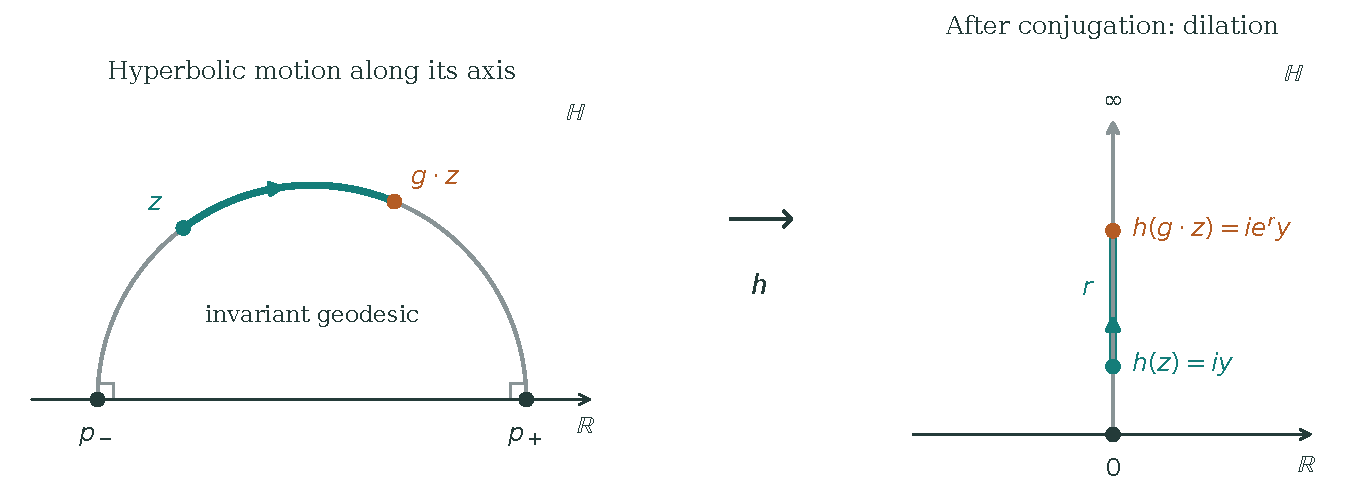
\includegraphics[width=\linewidth]{volumes/Volume01/A/chapters/Chapter01/sections/Section05/figures/translation-dilation.pdf}
\caption{Left: a hyperbolic transformation moves $z$ to $g\cdot z$ along the semicircular axis joining its repelling fixed point $p_-$ and attracting fixed point $p_+$. Right: $h$ sends these endpoints to $0$ and infinity and the axis to the positive imaginary axis. The corresponding points are $iy$ and $ie^r y$. Both highlighted segments have hyperbolic length $r$; corresponding endpoints have the same color.}
\label{hyperbolic.translation-dilation-diagram}
\end{figure}

We now measure how far a transformation must move a point, allowing the point to vary.

\begin{definition}[Translation length]\label{hyperbolic.translation-length}
For an effective transformation $\overline g\in\overline G$, define its translation length by
\begin{equation}\label{eq:translation-length}
 \ell(\overline g)=\inf_{z\in\mathbb H}d_{\mathbb H}(z,g\cdot z).
\end{equation}
Either lift $g$ or $-g$ gives the same action, so this definition is independent of that choice. The infimum is finite and nonnegative, since all displacements are nonnegative and the displacement of $i$ is finite. The identity has translation length zero.
\end{definition}

\begin{lemma}[Translation length is invariant under conjugacy]\label{hyperbolic.translation-length-conjugacy}
For $g,h\in G$, we have $\ell(\overline{hgh^{-1}})=\ell(\overline g)$. Moreover, $h$ carries the set of minimizing points for $g$ onto that for $hgh^{-1}$.
\end{lemma}

\begin{proof}
For every $w\in\mathbb H$, preservation of distance gives
\[
 d_{\mathbb H}(h\cdot w,(hgh^{-1})\cdot(h\cdot w))
 =d_{\mathbb H}(h\cdot w,h\cdot(g\cdot w))
 =d_{\mathbb H}(w,g\cdot w).
\]
As $w$ ranges over $\mathbb H$, so does $h\cdot w$. Thus the two sets of displacement values agree. Their infima in the definition of translation length \eqref{eq:translation-length} agree, and the displayed identity identifies exactly where those infima are attained.
\end{proof}

\begin{proposition}[Elliptic translation length]\label{hyperbolic.elliptic-length}
An elliptic transformation has translation length zero, attained precisely at its unique fixed point in $\mathbb H$.
\end{proposition}

\begin{proof}
If $p$ is its fixed point, then $d_{\mathbb H}(p,g\cdot p)=0$. Nonnegativity gives $\ell(\overline g)=0$. At any point $z$, the displacement is zero exactly when $g\cdot z=z$, so the \hyperref[hyperbolic.fixed-point-classification]{fixed-point classification} gives uniqueness of the minimizing point.
\end{proof}

\begin{proposition}[Parabolic translation length]\label{hyperbolic.parabolic-length}
A parabolic transformation has translation length zero, and the infimum is not attained at any point of $\mathbb H$.
\end{proposition}

\begin{proof}
By the \hyperref[hyperbolic.parabolic-normal-form]{parabolic normal form} and \hyperref[hyperbolic.translation-length-conjugacy]{conjugacy invariance}, it suffices to consider $z\mapsto z+t$ with $t\ne0$. For $z=x+iy$, the definition of the point-pair invariant gives
\[
 u(z,z+t)=\frac{|t|^2}{4y^2}.
\]
The point-pair distance identity \eqref{eq:point-pair-distance} therefore gives
\[
 d_{\mathbb H}(z,z+t)=2\operatorname{arsinh}\!\left(\frac{|t|}{2y}\right).
\]
Here we take the nonnegative square root in that identity and then invert $\sinh$ on $[0,\infty)$. As $y\to\infty$, this distance tends to zero by continuity of $\operatorname{arsinh}$ at $0$. Thus the infimum is zero. For every finite $y>0$ the argument $|t|/(2y)$ is positive, so the distance is positive and the infimum is never attained.
\end{proof}

\begin{proposition}[Hyperbolic translation length and axis]\label{hyperbolic.hyperbolic-length}
For a hyperbolic transformation,
\[
 \ell(\overline g)=2\operatorname{arcosh}\!\left(\frac{|\operatorname{tr}g|}{2}\right)>0.
\]
The minimizing points form the unique geodesic joining its two boundary fixed points, called its axis. The transformation translates along that axis by $\ell(\overline g)$.
\end{proposition}

\begin{proof}
First compute the displacement in the \hyperref[hyperbolic.hyperbolic-normal-form]{normal form} $z\mapsto e^r z$, with $r>0$. For $z=x+iy$,
\[
 \begin{aligned}
 u(z,e^r z)
 &=\frac{(e^r-1)^2(x^2+y^2)}{4e^r y^2}\\
 &=\sinh^2(r/2)\left(1+\frac{x^2}{y^2}\right).
 \end{aligned}
\]
The second equality uses $(e^r-1)/(2e^{r/2})=\sinh(r/2)$. This value is at least $\sinh^2(r/2)$, with equality exactly when $x=0$. The point-pair distance identity \eqref{eq:point-pair-distance}, together with strict increase of $s\mapsto\sinh^2(s/2)$ for $s\geq0$, now shows that
\[
 d_{\mathbb H}(z,e^r z)\geq r,
 \qquad d_{\mathbb H}(z,e^r z)=r\ \Longleftrightarrow\ x=0.
\]
Thus the translation length is $r$, and its minimizing points are precisely the imaginary axis. On that axis write $z=ie^s$. The dilation sends $ie^s$ to $ie^{s+r}$; the \hyperref[hyperbolic.vertical-geodesics]{vertical distance formula} makes $s$ an arclength coordinate, so the action is translation by $r$.

The determinant-one lift of this dilation has diagonal entries $e^{r/2}$ and $e^{-r/2}$, hence trace $2\cosh(r/2)$. Trace is unchanged by matrix conjugation, and its absolute value is unchanged by replacing a lift by its negative. Consequently
\[
 |\operatorname{tr}g|=2\cosh(r/2),
 \qquad r=2\operatorname{arcosh}\!\left(\frac{|\operatorname{tr}g|}{2}\right).
\]
Finally, \hyperref[hyperbolic.translation-length-conjugacy]{conjugacy invariance} carries the minimizing imaginary axis to the geodesic joining the original two boundary fixed points, while preserving its arclength and displacement. The \hyperref[hyperbolic.geodesics]{geodesic classification} gives uniqueness: two finite boundary endpoints determine the perpendicular semicircle, and one finite endpoint together with infinity determines a vertical line.
\end{proof}

\begin{remark}[Orientation is additional data]\label{hyperbolic.axis-orientation}
A hyperbolic transformation and its inverse have the same axis and translation length, but travel in opposite directions. Whether a later sum distinguishes these orientations depends on its indexing set and conjugacy relation. Likewise, a sum over matrices distinguishes $g$ from $-g$ unless the index set explicitly identifies them. Neither identification should be inferred from equality of geometric lengths alone.
\end{remark}
